% cpedoc.tex V2.0, 13 May 2010

\documentclass[times]{cpeauth}

\usepackage{moreverb}
\usepackage{xspace}

\newif\ifdraft
%\drafttrue
\ifdraft
\newcommand{\onote}[1]{ {\textcolor{cyan} { (***Ole: #1) }}}
\newcommand{\terminology}[1]{ {\textcolor{red} {(Terminology used: \textbf{#1}) }}}
\newcommand{\owave}[1]{ {\cyanuwave{#1}}}
\newcommand{\jwave}[1]{ {\reduwave{#1}}}
\newcommand{\alwave}[1]{ {\blueuwave{#1}}}
\newcommand{\jhanote}[1]{ {\textcolor{red} { ***shantenu: #1 }}}
\newcommand{\alnote}[1]{ {\textcolor{green} { ***andreL: #1 }}}
\newcommand{\mrnote}[1]{ {\textcolor{blue} { ***M says: #1 }}}
\newcommand{\smnote}[1]{ {\textcolor{brown} { ***sharath: #1 }}}
\newcommand{\pmnote}[1]{ {\textcolor{blue} { ***Pradeep: #1 }}}
\newcommand{\msnote}[1]{ {\textcolor{cyan} { ***mark: #1 }}}
\newcommand{\note}[1]{ {\textcolor{magenta} { ***Note: #1 }}}
\else
\newcommand{\onote}[1]{}
\newcommand{\terminology}[1]{}
\newcommand{\owave}[1]{#1}
\newcommand{\jwave}[1]{#1}
\newcommand{\alnote}[1]{}
\newcommand{\mrnote}[1]{}
\newcommand{\athotanote}[1]{}
\newcommand{\smnote}[1]{}
\newcommand{\pmnote}[1]{}
\newcommand{\jhanote}[1]{}
\newcommand{\msnote}[1]{}
\newcommand{\note}[1]{}
\fi

\usepackage{wrapfig}
\usepackage{color}
\usepackage{caption}
\usepackage{subcaption}

\usepackage{listings}  
\lstdefinestyle{myListing}{
  frame=single,   
  %float=t,
  language=C,       
  basicstyle=\ttfamily \footnotesize,
  breakautoindent=true,
  breaklines=true
  tabsize=2,
  captionpos=b,  
  aboveskip=0em,
  belowskip=-2em,
  %numbers=left, 
  %numberstyle=\tiny
}      

\lstdefinestyle{myPythonListing}{
  frame=single,   
  %float=t,
  language=Python,       
  basicstyle=\ttfamily \tiny,
  breakautoindent=true,
  breaklines=true
  tabsize=2,
  captionpos=b,  
  %numbers=left, 
  %numberstyle=\tiny
}

\newcommand{\cloud}{cloud\xspace}
\newcommand{\clouds}{clouds\xspace}
\newcommand{\pilot}{Pilot\xspace}
\newcommand{\pilots}{Pilots\xspace}
\newcommand{\pilotjob}{Pilot-Job\xspace}
\newcommand{\pilotjobs}{Pilot-Jobs\xspace}
\newcommand{\pilotcompute}{Pilot-Compute\xspace}
\newcommand{\pilotcomputes}{Pilot-Computes\xspace}
\newcommand{\pilotdata}{Pilot-Data\xspace}
\newcommand{\pilotdataservice}{Pilot-Data Service\xspace}
\newcommand{\pilotcomputeservice}{Pilot-Compute Service\xspace}
\newcommand{\computedataservice}{Compute-Data Service\xspace}
\newcommand{\pilotmapreduce}{PilotMapReduce\xspace}
\newcommand{\mrmg}{MR-Manager\xspace}
\newcommand{\pstar}{P*\xspace}
\newcommand{\pd}{PD\xspace}
\newcommand{\pj}{PJ\xspace}
\newcommand{\pjs}{PJs\xspace}
\newcommand{\pds}{Pilot Data Service\xspace}
\newcommand{\computeunit}{Compute-Unit\xspace}
\newcommand{\computeunits}{Compute-Units\xspace}
\newcommand{\dataunit}{Data-Unit\xspace}
\newcommand{\dataunits}{Data-Units\xspace}
\newcommand{\du}{DU\xspace}
\newcommand{\dus}{DUs\xspace}
\newcommand{\cu}{CU\xspace}
\newcommand{\cus}{CUs\xspace}
\newcommand{\su}{SU\xspace}
\newcommand{\sus}{SUs\xspace}
\newcommand{\schedulableunit}{Schedulable Unit\xspace}
\newcommand{\schedulableunits}{Schedulable Units\xspace}
\newcommand{\cc}{c\&c\xspace}
\newcommand{\CC}{C\&C\xspace}

\newcommand{\up}{\vspace*{-1em}}
\newcommand{\upp}{\vspace*{-0.5em}}

\usepackage[
%dvips,
colorlinks,bookmarksopen,bookmarksnumbered,citecolor=red,urlcolor=red]{hyperref}

\newcommand\BibTeX{{\rmfamily B\kern-.05em \textsc{i\kern-.025em b}\kern-.08em
T\kern-.1667em\lower.7ex\hbox{E}\kern-.125emX}}

\def\volumeyear{2012}

\begin{document}

\runningheads{A. Luckow et al.}{Pilot-Abstractions for Data-Intensive Cloud Applications}

\title{Pilot-Abstractions for Data-Intensive Cloud Applications}

%on Clouds and Grids}

%Extensible, Scalable, Interoperable 

\author{Andre Luckow, Pradeep Mantha, Melissa Romanus, Shantenu
  Jha\corrauth}

\address{Radical Research Group, Rutgers University}

\corraddr{Journals Production Department, John Wiley \& Sons, Ltd,
The Atrium, Southern Gate, Chichester, West Sussex, PO19~8SQ, UK.}

\begin{abstract}
% The data generated by scientific applications is experiencing an
% exponential growth. Addressing the consequences of this exponential
% growth has spawned the field of BigData. Given that data and compute
% resources cannot always be co-located, an important component of the
% BigData problem is how to utilize the efficient use of distributed
% resources so as to make meaningful sense of all of the data produced.
% In recent work we showed how MapReduce can be used to efficiently
% process distributed data across a distributed set of resources.
% Pilot-MapReduce (PMR) is a flexible, infrastructure-independent
% runtime environment for MapReduce. PMR is based on \pilot-abstractions
% for compute (Pilot-Jobs) and data (Pilot-Data). Pilot-Jobs are used to
% couple the map phase computation to the nearby source data, and
% Pilot-Data is used to move intermediate data using parallel data
% transfers to the reduce computation phase.

  The data generated by scientific applications is experiencing an
  exponential growth. The ability to analyze prodigious volumes of
  data requires flexible and efficient compute-data placement
  strategies.  This paper explores and establishes the use of
  \pilot-Abstractions as a runtime capability that supports a range of
  applications and analytical methods in a flexible and scalable
  fashion over a variety of execution environments. In particular, we
  focus on \pilotdata and the use of clouds as one element in a
  broader and heterogeneous distributed cyberinfrastructure.  To that
  end, we build upon existing capabilities of integrating MapReduce
  with \pilot-Abstractions, called Pilot-MapReduce (PMR) which % is
% based on \pilot-abstractions
%   for compute (Pilot-Jobs) and data (Pilot-Data) 
  provides a flexible, infrastructure-independent runtime environment
  for MapReduce.  Pilot-Jobs are used to couple the map phase
  computation to the nearby source data, and Pilot-Data is used to
  move intermediate data using parallel data transfers to the reduce
  computation phase.  In this paper, we discuss the generalization of
  the \pilot-Abstraction to clouds and investigate the use of PMR on a
  variety of cloud systems, as well as interoperably with other
  distributed resources.  We show how using \pilot-Abstractions, PMR
  enables the efficient processing of distributed data on
  heterogeneous distributed infrastructure including different
  academic and commercial clouds (e.g. Amazon EC2, Google Compute
  Engine and FutureGrid). We investigate the effectiveness of
  PMR-based applications on cloud infrastructure for % different
  next-generation gene sequencing applications.  The flexible runtime
  provided by the \pilot-Abstraction, helped establish PMR's
  effectiveness for distributed data scenarios on clusters that are
  nodes on a WAN. Given the different network characteristics within
  clouds, we investigate whether performance determinants for
  clusters, are valid for clouds. \jhanote{we should refine the
  previous sentence} Our analysis covers multiple scenarios exposing
  the different (typical) trade-offs: e.g., the overhead times in
  spawning virtual machines, different storage types, geographic
  distribution, and establishes that the \pilots provide a powerful
  abstraction for \clouds as well.
  %We analyze different resource and MapReduce configurations, such as
  %both hierarchical and distributed MapReduce using an NGS
  %application. \jhanote{Not sure the previous is
  %  true}. 
\end{abstract}

\keywords{Cloud Computing, MapReduce, Grid Computing, Data-Intensive}

\maketitle


\vspace{-6pt}

\section{Introduction}
\vspace{-2pt}

% Intro Big Data

An important trend is the emergence of large-volume of data, rich in
semantics, complexity and information. One attribute, often overlooked
is that the prodigious amounts of data is fundamentally distributed --
often due to source of production or location of
consumption/analysis. In general, distributed data has become a
critical factor in many science disciplines \cite{fourthparadigm},
e. g. in the areas of fusion energy (ITER), bioinformatics
(metagenomics), climate (Earth System Grid), and astronomy
(LSST)~\cite{Jha:2011fk}. In addition to efficient algorithms and
methods, an increasing number of these applications need to
effectively utilize a diverse range of infrastructure, including
clouds in addition to traditional cyberinfrastructure.  Furthermore,
these infrastructure are distributed and even though they are still
evolving they are often disjoint.

% And cloud trends

Interestingly even though clouds have their origins in enterprise
computing, they provide novel opportunities for science \& engineering
applications.  As has been extensively documented~\cite{Jha:2010kx},
clouds offer a relatively simple, easy-to-use environment with respect
to resource management, capacity planning capabilities, software
environment \& control etc.  An interesting capability of clouds is
the possibility to bootstrap custom runtime environments, which is
often difficult with grids. For example, a number of applications are
difficult to build, due to runtime dependencies, or complicated
non-portable build systems. This provides an additional rationale for
cloud environments. After an application environment is created once,
it can be loaded on to various systems, working around issues related
to portability on the physical systems. Furthermore, clouds provide
greater scheduling flexibility, for example, when the set of resources
needed to run an application changes (perhaps rapidly), the resources
employed can actually be changed (new resources can be added, or
existing resources can be removed from the pool used by the job).

We believe there are three primary architectures for data-intensive
analytics: (i) localize all data into a cloud (or a large analytical
engine), (ii) decompose and distribute data to as many
computing/analytical engines are available (this incidentally is the
paradigm employed by particle physics for the discovery of the Higgs),
and (iii) a hybrid and hierarchy of the above two paradigms, wherein
data is decomposed and committed to several infrastructure, which in
turn could be a combination of either of the first two paradigms.
Although it is obvious that large-volumes of data can be poured into a
cloud, there are limitations to the scalability or validity of this
model, viz., what if data-volumes are too large to move, or have
constraints on the ability to move centrally (say due to security or
privacy concerns). In other words, can clouds also be used for the
second and third architectural paradigms, and if so,
how? % Although it is obvious that large-volumes of data can be
% poured into a cloud, there are limitations to the scalability or
% validity of this model, viz., what if data-volumes are too large to
% move, or have constraints on the ability to move centrally (say due to
% security or privacy concerns)? 
This is not unrelated to runtime capabilities which enable applications
to utilize any of the three architectures as needed (viz., based upon
data size and resource availability).


% i.\,e.\ the number of applications that need to efficiently support
% {\it Runtime Environment:} \alnote{we could also make the case that
%   the cloud landscape is highly fragmented by itself...}

Even whilst the macroscopic architecture for data-intensive computing
and the relationship of clouds to other elements of the distributed
cyberinfrastructure is still converging, there is churn within clouds,
i.e., the cloud capability and infrastructure landscape has become
highly fragmented. Amidst this fragmentation, 
the case for cloud interoperability and cloud-grid interoperability
can be made. % Motivated by the need for such interoperability an
% important question that arises is how can this be provided in a
% extensible and flexible fashion. 
How can such interoperability be provided in an extensible and
flexible fashion?  The answer is partly dependent upon the level and
type of interoperability (application-level, service-level etc)
desired, but one route to interoperability definitely arises from a
unified model of runtime execution.  Are there abstractions that can
provide such unification?

% Viewed from another perspective,
% much has been said and incorrectly assumed about the ``elastic''
% properties of clouds. Clouds do not provide infinite and immediate
% access to resources, at least not with at the same level of
% quality/performance. The putative illusion of infinite elasticity is a
% consequence of system-level multiplexing.  We posit that such
% ``elastic'' characteristics can also be provided by
% % pilot-abstractions
% runtimes which support qualitatively similar dynamic execution modes.


The high-level motivating question for this work thus emerges: How can
clouds be used to support the requirements of distributed
data-intensive applications?  Whereas any answer to the above, is
bound to be complex and constrained, we concentrate on two components:
(i) architecture of the data-cyberinfrastructure and (ii) runtime
environments. Thus, the motivating question can be positioned as, are
there runtime capabilities that provide the abstractions required for
flexible execution whilst supporting different data-analytic
architectural paradigms?  We posit that \pilot-Abstractions provide
precisely such a unification of the runtime/execution model with the
architectural flexibility required and thus can meet the requirements
of data-intensive applications.

% as well as an answer to the earlier posed question of how
% the use of clouds can be extended to
% So the underlying intellectual issue motivating this work
% This points to the role of flexible runtime environments

\pilotjobs have proven to be a successful abstraction for distributed
and high-performance applications, whereby they decouple the workload
specification from its execution. A \pilotjob provides the ability to
utilize a placeholder job as a container for a dynamically determined
set of compute tasks. Recent work on the P* (Pstar)
Model~\cite{pstar12} has provided a formal theoretical basis for
Pilot-Jobs and provided a conceptual framework upon which to analyze
and compare distinct implementations. Significantly, the P* Model
provided a symmetrical but logical extension to Pilot-Jobs to data,
and introduced the concept of Pilot-Data, which akin to Pilot-Jobs for
computational tasks, provides an efficient and extensible route to
decoupling the ultimate location of data storage and/or consumption
from its production.  

\begin{figure}[t] 
\centering
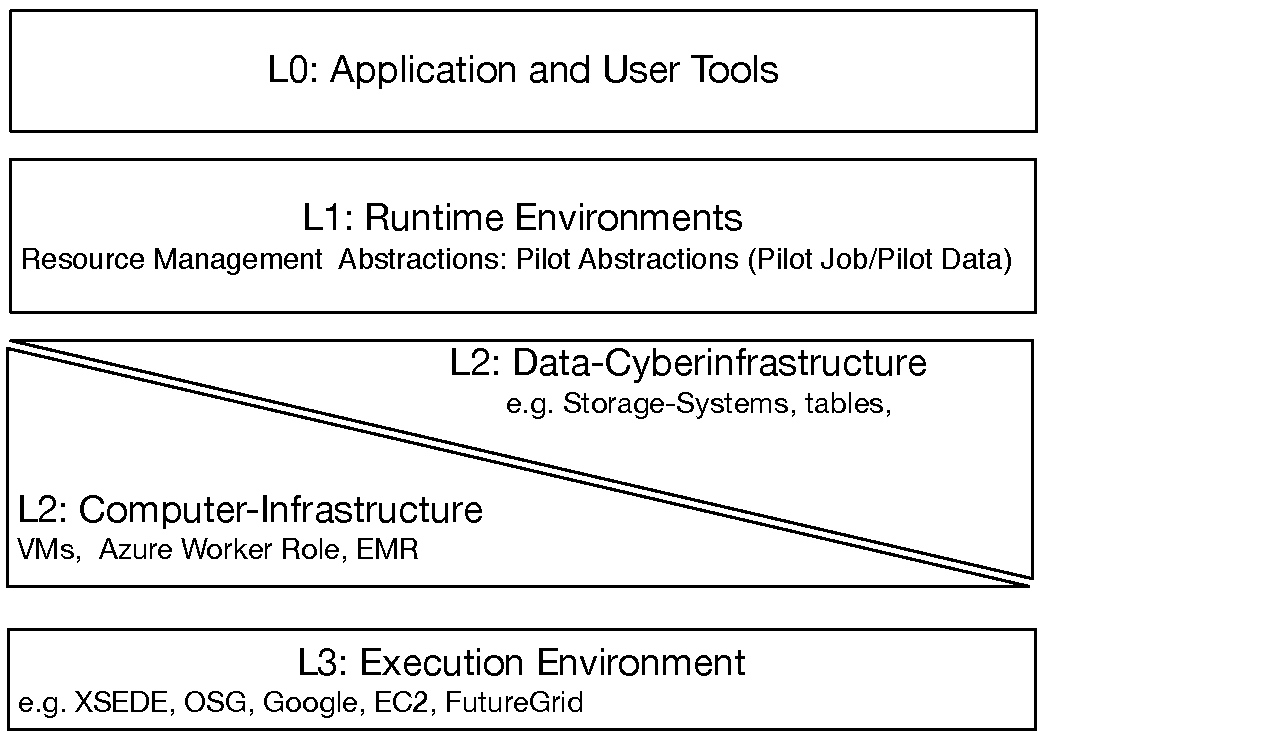
\includegraphics[width=0.6\textwidth]{figures/data-intensive-arch.pdf}
\caption{\textbf{\pilot-Abstraction and Data-Cyberinfrastructure:} High-level schematic of how different components referred to
  in the paper relate to each other, and in particular how
  \pilot-Abstractions place within a broader data-cyberinfrastructure.}
\label{fig:figures_arch}
\end{figure}

We have previously discussed the effectiveness of \pilot-Abstractions
for the second architectural paradigm~\cite{pstar12}.  A primary contribution
of this work is in establishing \pilot-Abstractions as a valid
resource and runtime abstraction for data-intensive applications for
clouds for all three architectural paradigms.  Traditionally
compute-data cyberinfrastructure was integrated, or at least the data
cyberinfrastrucutre (such as storage, access mechanisms etc.)  were
pretty much determined and constrained by the compute environment.
Probably in response to increasing data volumes and challenges
inherent, a recent trend is a decoupling between the two, i.\,e.,
data-cyberinfrastructure is often an independent degree-of-freedom and
importantly often the primary degree-of-freedom, i.e.,
data-cyberinfrastructure considerations come together if not before
compute considerations.  This is schematically represented in the
level diagram by a logical separation of the same level (L2) in
Figure~\ref{fig:figures_arch}.  Thus it is important that any
effective runtime abstraction be able to support a diverse range of
data-cyberinfrastucture and data localization models imposed by them.
In this work, we establish that \pilot-Abstractions provide a common
runtime/execution model across the range of proliferating compute and
data-cyberinfrastructure.  Furthermore, we illustrates an
interoperable and scalable approaches to providing dynamic resource
utilization (often loosely called ``elastic resource utilization'').

After discussing relevant and prior work in the next section, we
present a brief discussion of the landscape of elements comprising
cloud cyberinfrastructure. Any effective runtime abstraction must be
able to support applications against the rich and dynamic landscape.
Section 4 provides a conceptual extension of the \pilot-Abstraction to
clouds, we propose that it provides a runtime abstraction which
supports interoperability across a diverse and dynamic
cyberinfrastructure landscape.  Section 4 also provides an overview of
\pilotdata and affinity, and how these concepts apply to cloud
infrastructure. % In addition to providing
% validation of
Section 5 discusses how the \pilot-Abstraction has been used to
support flexible and extensible implementations of MapReduce -- a
well-known pattern/programing model for data-intensive applications.
The integration of MapReduce and \pilot-Abstraction, referred to as
\pilotmapreduce, paves the way for uniform execution environment for
grids and clouds, and thereby sets the stage for common scheduling,
localization and optimization techniques.  In Section 6, we design and
discuss a set of experiments with the aim of establishing
\pilot-Abstractions as a runtime abstraction as measured by a set of
objectives, viz., validity, interoperability and ability to support
application/application-level patterns.

% although relevant to all three paradigms, in this paper we will focus
% on techniques and abstractions primarily for the second and third
% paradigms.
 

% With this capabilities, clouds provide an interesting complement to
% existing CI.  The ability to exploit these attributes will lead to
% applications with new and interesting usage modes and dynamic
% execution on clouds and therefore new application
% capabilities
%Although there are many~\cite{Jha:2010kx, fourthparadigm}. 

%\subsection*{The Case for Distributed, Data-intensive Computing}

% \jhanote{Talk about how runtime environment must support a wide range
%   of data and compute cyberinfrastucutre, along different
%   architectures (configurations), with minimal distribution. Reference
%   Figure 1.}
% For example, given an application and data-volumes, which
% distribution/analysis paradigms is advisable?  (ii) effective
% distribution strategies.


% \begin{itemize}
% 	\item choosing the right cloud... 
% 	\item how to couple different clouds
% 	\item transport in and out to cloud
% 	\item support late-binding: late binding as a fundamental attribute in 
% 	distributed systems
% \end{itemize}

% Application perspective versus Infrastructure perspective: (I)
% Application Motivation/Challenges: Scaling data intensive
% applications - Why is this a problem? Any real application requires
% this problem to be solved?  - CMS, Atlas generates PBs of data/ day.
% (II) Infrastructure Motivation: Emerging infrastructure, data
% oriented infrastructure, scalability of infrastructure, possibly
% better abstractions and capabilities.

% \begin{verbatim}
% Note our focus and context: (i) distributed data scenarios (ii) pilot
%  abstraction to address heterogeneity, scalability and extensibilty
% \end{verbatim}

% Some Research Questions: (i) How does Pilot-Abstraction work in the
%  clouds (we've addressed pilot-jobs before, now focus on pilot-data)
%  (ii) how to address data distribution in the cloud? (iii) cloud data
%  localization requirements: how and when does that become a barrier?
%  (iv) related to previous, Can we say something when to use cloud or
%  When Grid?

% \jhanote{Other Issues worth mentioning: not sure what these are tying
%  to say: Does minimizing queue wait time, distributed nature of
%  Pilot-abstractions motivate Domain Scientists to use freely available
%  Grid resources?  Waiting time and cost increases as Number of
%  instances required increase?  HOw is it beneficial than Grids?}

%\pmnote{ Scientists believe clouds provide computing infrastructure on
%  demand with minimal or negligible waiting time..  Production
%  cyberinfrastructures involve waiting time if they don't take
%  advantage of Pilot abstractions...  So, what I want to say is-
%  scientists are ignoring existing abstractions and simply moving to
%  cloud.. Is that because of hype? }

%\note{Why Domain scientists are moving to cloud? Hype? Due to
%  non-availability of necessary simple abstractions to scale
%  applications on Grid?}  \pmnote{ I mean , Given the success the
%  Pilot abstractions on Grids , Domain scientists should start using
% Pilot abstractions rather than using on demand cloud services -
%  which are expensive - I think its an opportunity to exploit the
%  importance of BigJob and SAGA; Can we mention some usecases where
%  PJ's effectively supported real science(Tom Bishop usecase)?  I
%  think as PJ's popularity increases - requirement to use clouds
%  decreases ( since no waiting time between compute units) )}
%\jhanote{Pradeep: please read text now. Does it address some of your
% questions of why scientists are moving to clouds?}  \pmnote{Does
%  clouds support real science.}\jhanote{Some types yes definitely. Not
%  all types that is also for sure!}


%\note{Not in scope any more: Why Iterative MapReduce?What
%  Application?  ( k-means?)Why k-means?  - twister mapreduce used
%  k-means?  - k-means implemented using windows azure}




\section{Related Work}


\subsubsection*{Related Work:} 


\mrnote{Should I mention pilot-jobs and the first pilot-job implementation being condor glide-in?}
\jhanote{Btw, I hope we're not going to use bullet points in final version?}

%\note{Melissa}
\pilotjobs have existed on grid infrastructures for some time. Batch queuing
systems on the existing grid hardware drove the desire for user-level control
of tasks and ease of use of job descriptions for data driven applications.
\pilotjobs provide the ability to distribute workload across multiple systems
and provide an easy way to schedule many jobs at one time. The first such
implementation of a \pilotjob was Condor Glide-in~\cite{glidein}. A Glide-in
daemon can pull Condor binaries to a compute node. This compute node then
becomes available in a given Condor pool as a resource. Jobs can then be run
on the pool of compute nodes.

Since the notion of \pilotjobs saw such promising uptake on grids, it
was natural that this work be explored in its extension to clouds. An
infrastructure requirement out of CERN drove the creation of
CoPilot~\cite{copilot-tr}, which acts as a layer on top of existing
grid/batch systems to allow job submission to clouds such as Amazon
EC2 or Scientific Clouds. The creation of CoPilot was driven from the
high energy physics community having requirements for cloud/grid
interoperability. CoPilot uses XMPP messaging to communicate between
the VMs and the grid infrastructure. It is based more on the actual
submission of jobs and focuses less on user-level control and
application-level programming than SAGA BigJob.

The Coaster system~\cite{coasters} is another \pilotjob implementation which
has been shown to work in both cloud and grid environments. Using the Coaster
service, one executes a master on the head node, and the Coaster workers run
on compute nodes to execute jobs sounds at least vaguely familiar. Coasters
offers a zero-install feature in which it deploys itself and installs itself
from the head node and onto the virtual machines without needing any prior
installation on the machine. In cloud mode, Coasters does require installation
to a head node. While SAGA BigJob uses SAGA to connect to middleware, Coasters
uses the CoG kit abstraction library for gram, ssh, Condor, PBS, SGE support.
While Coasters has been shown to be effective for clouds, grids, and clusters
independently, its notion of \pilotjobs has not been shown interoperably
across both clouds and grids.
 
The Venus-C Generic Worker~\cite{venusc-generic-worker} is a cloud-only
approach to \pilotjobs from Microsoft. Venus-C is built upon Microsoft Azure,
but in order to create a layer of abstraction above the inner workings of the
cloud, the idea of a Generic Worker was born. The idea behind the Generic
Worker was to allow scientists to do their science without requiring knowledge
of backend HPC systems by offering e-Science as a service. Venus-C has not
been shown to work with grids, because its main objective is to get scientists
using cloud infrastructure instead. While the notion of moving to the cloud
for data-driven science is an important one, many existing
cyberinfrastructures still have powerful grid computers that can also be
leveraged to assist with the data-driven computations.

\subsubsection*{Prior Work:}
% %\alnote{needs to be aligned with 5; add paragraph on P*, u% \begin{itemize}

Whereas we will discuss in greater Sections 4 and 5 some of the
concepts upon which this paper is built, for completeness we briefly
outline them here.

\noindent {\it Towards a Theoretical Model of Pilot-Jobs and
  Interoperable Implementations: } The seamless uptake of distributed
infrastructures by scientific applications has been limited by the
lack of pervasive and simple-to-use abstractions at multiple levels –
at the development, deployment and execution stages. Of all the
abstractions proposed to support effective distributed resource
utilization, a survey of actual usage suggested that \pilotjobs were
arguably one of the most widely-used distributed computing
abstractions – as measured by the number and types of applications
that use them, as well as the number of production distributed
cyberinfrastructures that support them.  Our initial
investigation~\cite{Luckow:2008la} into \pilot-Abstractions
was motivated by the desire to provide a single \pilotjob framework
that would work over heterogeneous and myriad types of grid middleware.

This led to BigJob~\cite{saga_bigjob_condor_cloud} -- a SAGA-based
\pilotjob, which was used to support a range of applications, ranging
from uncoupled ensembles of molecular dynamics (MD)
simulations~\cite{saga_bigjob_condor_cloud}, to Ensemble-Kalman filter
based applications~\cite{gmac09} with global synchronization to
loosely-coupled MD simulations with pair-wise
synchronization~\cite{async_repex11}.  Although BigJob provided the
syntactical uniformity, i.e., a common API and framework for different
grids, our experience led us to understand that different \pilotjobs
had different semantics and capabilities, and made vast if not
inconsistent assumptions of applications/users. This motivated our
efforts in search of a common minimally complete model of \pilotjobs,
and resulted in the \pstar model~\cite{pstar12}.

Once a common and uniform conceptual model was available, the notion
of \pilotdata was conceived using the power of symmetry, i.e., the
notion of \pilotdata was as fundamental to dynamic data placement and
scheduling as \pilotjobs was to computational tasks. As a measure of
validity, the \pstar model was amenable and easily extensible to
\pilotdata.  The consistent and symmetrical treatment of data and
compute in the model led to the generalization of the model as the
{\it P* Model of Pilot Abstractions}.

% We In spite of broad uptake, there does not exist a well-defined,
% unifying conceptual model of Pilot-Jobs which can be used to define,
% compare and contrast different implementations. Often Pilot-Job
% implementations are strongly coupled to the distributed
% cyberinfrastructure they were originally designed for. These factors
% present a barrier to extensibility and interoperability.  The P* Model
% provides a conceptual basis to compare and contrast different PJ
% frameworks. Natural and logical extension to the base P* Model lead to
% an abstraction analogous to Pilot-Job: the Pilot-Data (PD)
% abstraction.

{\it Pilot-MapReduce}: Following on the foundation laid by the P*
Model of Pilot abstractions, a natural logical next step was to
investigate if the capabilities of \pilot-Abstractions could be used
to support agile and dynamic execution modes for application and
application-patterns?  This was in-turn motivated by the observation
that the MapReduce programming model is a popular solution for
distributed data processing and involves map and reduce (compute)
phases, and a shuffle (data movement) phase. However, traditional
MapReduce implementations like Hadoop are typically designed for
single clusters and when scaled across widely distributed clusters
lead to performance problems.  Furthermore, when working in a
distributed data context, a static resource assignment for MapReduce
is very constraining.  Could the use of dynamic runtime environment
such as that provided by \pilot-Abstractions overcome some of the
traditional limitations of MapReduce, as well as the policies of the
typical clusters they execute on?  This led to the development of a
Pilot abstractions based
MapReduce~\cite{Mantha:2012:PEF:2287016.2287020} programming model ---
\pilotmapreduce, and an investigation into its suitability for
distributed data analysis.  \pilotmapreduce decouples the
logic/pattern of MapReduce from the actual management of the
distributed compute, data and network resources. By decoupling job
scheduling and monitoring from the resource management,
\pilotmapreduce efficiently reuses the resource management and
late-binding capabilities of BigJob and BigData, which are SAGA based
Pilot-Job and Pilot-Data implementations.

% we provides a flexible and effective management of compute and data
% on distributed CyberInfrastructures.  The P* abstractions support
% management of DCI by various data and compute intensive programming
% models.  Deployment of Hadoop cluster on shared dynamic resource
% pool also involves manual management of compute and data resources
% and managing workflows involving MapReduce execution patterns
% becomes tedious. Policies of cyberInfrastructures doesn't allow to
% execute Hadoop on more than one cluster.  Attempts to overcome such
% limitations of traditional implementations and capabilities of P*
% Model motivated to

\section{Cloud-based Infrastructures for Data-Intensive Applications}

% \jhanote{Do we need to proffer a defintion of cloud computing? And if
%   so, is this the right place?} At a high level, cloud computing is
% defined by Mell/Grance~\cite{nist_cloud} as a model for enabling
% convenient, on-demand network access to a shared pool of configurable
% computing resources (e.g., networks, servers, storage, applications,
% and services) that can be rapidly provisioned and released with
% minimal management effort or service provider interaction.
% \jhanote{In the above, is it network access or networked access?}\alnote{took 
% the definition more or less from the book chapter. networked sounds also 
% good.}

Whereas a cloud can be described on the basis of how (i.e., at what
level the cloud as a service is provided), we will focus on the the
specific elements that comprise the data-cyberinfrastructure
sub-system (see Fig.~\ref{fig:figures_arch}).  This is motivated by
the fact that different cloud services that aim to support Big Data
analytics have emerged.  The foundation for many of the different Big
Data offerings are different kind of storage services available,
typically at the IaaS level.  However, in order to appreciate the
landscape of these cloud-based data-cyberinfrastructure and how they
are provided, for completeness we review some established cloud
taxonomy and terminology.

\subsubsection*{Cloud Taxonomies: }
There are multiple possible cloud taxonomical classifications. One
approach classifies clouds as a service and uses the nature of the
service as the basis. Using the ``as-a-Service'' taxonomy, clouds are
classified into three categories: Software as a Service (SaaS),
platform as a service (PaaS), and Infrastructure as a Service
(IaaS)~\cite{Jha:2010kx}. The infrastructure-as-a-service (IaaS) layer
provides low-level, typically virtualized data and compute resources.
Computational resources are typically represented as virtual machines
instances. Examples for IaaS services are Amazon EC2~\cite{amazon_ec2}
and S3~\cite{amazons3} as well as the new Google Compute Engine
(GCE)~\cite{gce} service. PaaS services provide a higher-level
capabilities, such as controlled runtime environments for web
applications, task ensembles or MapReduce.  Example of PaaS services
are: Azure Web and Worker Roles, Google's App Engine,
BigQuery~\cite{google-bigquery} and Prediction
API~\cite{google-predication-api}, and Amazon Elastic
MapReduce~\cite{amazonemr}.


% Amazon API
% GData API
% OpenStack API
% OCCI
% 
% \begin{itemize}
% 	\item Resource Model
% 	\item Provisioning Model
% 	\item Business Model
% \end{itemize}


% Commercial Clouds vs. Science Clouds

Adjunct to the above classification, Clouds can also be classified
according to their deployment model into public and private
clouds. Frameworks such as OpenStack~\cite{openstack} and
Eucalyptus~\cite{euca} aim to provide a framework for building a
private cloud environment which similar capabilities as EC2 and
S3. FutureGrid's cloud environment currently supports both
framework. Currently, new science cloud infrastructures, e.\,g.\
FutureGrid~\cite{futuregrid}, are being developed and existing
production infrastructures are being expanded with cloud capabilities,
e.\,g.\ EGI~\cite{egi-cloud}. While the focus of many science clouds
is currently mainly on IaaS, there are several attempts in providing
high-level PaaS services: FutureGrid e.\,g.\ offers Hadoop
appliances~\cite{2016793} and Venus-C~\cite{venusc-generic-worker}
provides a generalized worker role service (similar to the Azure
Worker Role).



% \alnote{merge 3.1 and 3.2
\subsubsection*{Cloud Data-Infrastructure: }
The storage services typically have different characteristics, i.\,e.\
they usually differ in their read and/or write performance, supported
data volumes, interfaces \& semantics, consistency guarantees, degree
of replication, reliability, scalability etc.
%Many clouds offers various kinds of storage services with different
%characteristics, e.\,g.\ these services usually differ in their read
%and/or write performance, supported data volumes, interfaces,
%reliability and scalability
(see Baron~\cite{baron2010} for an overview of Amazon's storage
services). While clouds often provide storage services with different
semantics and at different levels of abstractions (including
e.\,g.\ relation databases), in the following we focus on general
file-based storage types. In general, file-based cloud storage can be
classified as follows: (i) local storage refers to local hard disk
directly attached to the compute resource (typically a VM); (ii)
remote storage refers to different forms of distributed (possible
parallel) filesystems than can be attached to a VM either as block
storage device or NAS. Both type (i) and (ii) storage is commonly
integrated via the Linux virtual filesystem layer and thus, is
suitable in particular for legacy, file-based applications.

A novel type of storage introduced by cloud environments are (iii)
object stores, which are highly distributed storage systems that can
potentially spawn across multiple data centers. Object stores are
optimized primarily for ``write once, read many'' workloads and can
support massive volumes of data with their scale-out
architectures. For example, Amazon S3 automatically replicates data
across multiple data centers within a region. These kind of stores are
not suitable for all workloads (e.\,g.\ traditional, transactional
workloads). On the other hand, typical Big Data workloads that (i)
require the storage of large volumes of data and (ii) are
characterized by a large amount of reads are particularly suitable for
such stores. Access to such storage systems is via a common -- often
simplified -- namespace and API. For example, cloud systems, such as
the Azure Blob Storage, Amazon S3 and Google Storage, provide only a
namespace with a 1-level hierarchy. This means that applications need
to be adapted, in order to benefit from object
storage. The most widely used object stores are: Amazon
S3~\cite{amazons3}, Azure Storage~\cite{azure-blob-storage} and Google
Cloud Storage~\cite{google-storage}. In addition, both Eucalyptus and
OpenStack provide an object store: Eucalyptus Walrus~\cite{walrus} and
OpenStack Swift~\cite{openstack-swift}. A major limiting factor, is
the necessity to ingest large volumes of data over the WAN. Large
volume data transfer are associated with high costs and unpredictable
and/or unacceptable performance.

Table~\ref{tab:storage-systems} shows an overview of distributed storage
systems. In addition to the described object stores and local storage that is
directly attached to the VM, each cloud infrastructure provides several
further storage options. The focus of this analysis are file-based storage
systems. Structured storage types (e.g. relational databases) and key-/values
stores are not considered. Azure Drive~\cite{azure-drive}, Amazon
EBS~\cite{baron2010} and Google Compute Engine Disks~\cite{gce_disks} are
comparable block-based storage service that provide storage that can directly
be attached as device to a VM. Some services support special features, e.\,g.\
Azure Drive can be backed by both page and block blobs optimizing for random
respectively sequential access; Amazon EBS supports guaranteed I/O on EBS
volumes. Similar, services exist for both Eucalyptus and OpenStack: Eucalyptus
Block Storage~\cite{euca-block} and Nova Volume~\cite{nova-volume}.

On traditional HPC and HTC infrastructure the notion of dynamically
provisioned storage does not exist. However, in particular HPC
infrastructures, such as XSEDE, typically provides access to a parallel
filesystem, such as Lustre~\cite{lustre} or
GPFS~\cite{Schmuck:2002:GSF:1083323.1083349}. On the Open Science Grid (OSG)
only local storage is available. In addition, both infrastructures provide or
are going to deploy distributed storage services: The Global Federated File
System (GFFS)~\cite{gffs} is currently evaluated in the context of XSEDE. GFFS
provides a global namespace on top of various XSEDE storage resources. The
system handles file movement, replication etc. transparently. OSG deploys 
several SRM-based storage services~\cite{srm-ogf}.



\begin{table}[t]
\centering
\begin{tabular}{|p{1.7cm}|p{1.3cm}|p{1.3cm}|p{1.3cm}|p{1.4cm}|p{1.4cm}|p{1.3cm}|p{1.2cm}|}
	\hline
	\textbf{Storage Type} &\textbf{Azure} &\textbf{Amazon} &\textbf{Google} &\textbf{Open\-Stack} &\textbf{Euca\-lyptus} &\textbf{XSEDE}  &\textbf{OSG} \\
	\hline
	Local	&yes &yes &yes &yes &yes &yes &yes\\
	\hline
	Remote &Azure Drive &EBS &GCE Disks &Nova Volumes &EUCA Block Storage &Lustre, GPFS 
	&no\\
	\hline
	Distributed Storage &Azure Blob Storage &S3 &Google Storage &Swift & Walrus &GFFS
	 &SRM\\
	\hline	
\end{tabular}
\caption{\textbf{Storage Types Supported by the Different Infrastructures:} 
Each infrastructure supports various storage options. Most commonly, storage 
is mounted as a local or remote filesystem. Distributed object storage 
provides some interesting characteristics for data-intensive applications. 
\label{tab:storage-systems}}
\end{table}

% In general, the following strategies for managing the distribution of compute 
% and data in cloud/grid environments exist~\cite{jha-katz-2013}:
% \begin{itemize}
% \item A: Data is naturally distributed, processing happens locally to
% 	the data.
% \item B: Data is originally localized, but the data needs to be distributed to 		
% 	match the distribution of compute resources.
% \item C: Data is moved so as to be localized (i.e., raw data is moved)
% \end{itemize}
% We want to use hybrid infrastructures in all of these modes.

{\it Data Management:} As explained before, various strategies for
managing data in distributed environments exist. The most common
approach in the context of clouds is the localization of all data,
i.\,e.\ the application data is initially pushed to a cloud storage
service, such Amazon S3, Google Storage and Azure Storage.  These
service, such as S3, are well suited for storing large amounts of data
and support typical data-intensive workloads (e.\,g.\ with a lot of
sequential reads). Often, cloud providers make different type of data
sets (e.\,g.\ the 1000 genome dataset) directly accessible from their
central object store. By eliminating the initial data movement, the
entry barrier to running computations on this data in the cloud is
significantly decreased.

Often, data is too large to move and thus, must either be
pre-processed or completely processed before it can be moved. Even within
single clouds, the management of data across different regions is challenging, 
e.\,g.\ Amazon S3  replicates data geographically but only within a single
region.

While some cloud services that support a high degree of geographic
distribution have emerged, e.\,g.\ content delivery services such as
Akamai and Amazon CloudFront, dealing with geographically distributed
data remains a challenge. However, both Google and Facebook internally
deploy systems that supports the management of large data volumes
across multiple, geographically dispersed locations. Both Google
Spanner~\cite{dean09} and Facebook Prism~\cite{Metz12} aim to provide
one logical namespace and handle the automatic replication and
movement of data. However, these capabilities are currently not
available as external cloud services. If an application requires such
capabilities, it needs to implement these manually.  In this paper we
show how \pilot-Abstractions can help manage data dynamically and
geographically distributed data.

\subsubsection*{Cloud Compute Infrastructure:} In addition to storage systems,
there are other cloud infrastructures that although important in
understanding cloud capabilities and applications that can be
supported. For example, the availability of {\it queues} provides
agile and effective approaches to distributed coordination.
Furthermore, Hadoop~\cite{hadoop} has become an important building
block for many data-intensive applications in clouds. Amazon
e.\,g.\ offers with Elastic MapReduce (EMR)~\cite{amazonemr} a pay per
use MapReduce clusters. EMR is based on Amazon EC2 and S3 and supports
out-of-the-box both the open source and the MapR Hadoop
distribution. It includes, not only the Hadoop core, but also Hive,
Pig and HBase. Amazon provides a file system adaptor for S3,
i.\,e.\ data can be streamed from S3 into Hadoop. Microsoft provides a
similar service based on the Hortonworks Hadoop
platform~\cite{hortonworks} called to Hadoop on
Azure~\cite{hadooponazure}. Also, various markets for data in the
cloud have emerged. Cloud providers, such as Amazon and Microsoft
published various scientific data set in these markets. Amazon
e.\,g.\ provides access to 200\,TB of data of the 1000 genome
project~\cite{amazon-1000genomes} and the CloudBurst Hadoop
application~\cite{schatz2009}. 


\subsubsection*{Cloud Applications:}
While cloud environments have traditionally deployed in commercial
settings, more and more science applications utilize to some extend
cloud resources or are natively developed for clouds. While
traditional HPC applications -- often based on MPI -- show limitations
in cloud
environments~\cite{Evangelinos2008,Mehrotra:2012:PEA:2287036.2287045},
there is a broad class of loosely-coupled applications that is
well-suited for clouds~\cite{1851544,Sehgal2011590}. There is a large
class of data-intensive applications that is loosely coupled and thus
very well-suitable for cloud environments, e.\,g.\ genome sequencing
applications or applications based on the replica-exchange
algorithm~\cite{bigjob_cloudcom10}.



\section{Pilot-Abstractions for Clouds}

% \alnote{the introduction to this section is a bit long. Maybe it makes
%   sense to extract some parts like the P* model into a separate
%   subsection}\jhanote{admitted its long. trying to fix}

\pilot-Abstractions provide a suitable means to marshall heterogeneous
sets of both compute and data resources and support the efficient
utilization of different kinds of commercial as well science cloud
resources.  \pilot-Abstraction have been extensively used on both HPC
and HTC infrastructures for a range of application scenarios as a
resource management abstraction to, (i) improve the utilization of
resources, (ii) to reduce wait times of a collection of tasks, (iii)
to facilitate bulk or high-throughput simulations where multiple jobs
need to be submitted which would otherwise saturate the queuing
system, and (iv) as a basis to implement application specific
execution, scheduling and policy decisions (see
Figure~\ref{fig:figures_pilot-abstractions}).
 
%  \subsection*{Scalable and Flexible Resource Managment Capabilities for
%    Clouds}

As alluded to in the introduction, there are many reasons motivating
the exploration and extension of \pilot-Abstractions for clouds.
% Independent of application motivations, here we focus on how \pilots
% provide a runtime environment that supports ``native capabiliites'' of
% clouds such as ``cloud bursting'', and also as a way of achieving
% interoperability. The same capability also makes \pilots suitable
% abstraction for building higher-level application capabilities, such
% as \pilotmapreduce.
\pilotjobs map well to IaaS cloud systems, wherein a \pilot can
marshall multiple VMs, possibly of different characteristics and
performance capabilities; an agent which pulls and executes tasks is
deployed on each VM. Ultimately, there is a decoupling between task
specification and resource assignment, with the \pilot-Manager or an
equivalent cloud-entity carrying out the mapping using
dynamic/real-time information.  Given the above, not surprisingly, the
\pilotjobs concept has already been applied to clouds; for example,
PaaS cloud systems, such as Venus-C
(Azure)~\cite{venusc-generic-worker}, support the notion of Generic
Workers (worker role) which are conceptually similar to \pilots in
that they pull tasks (application workload) from a {\it central
  repository} when the environment is available.


% Using the compute/data abstraction of \pilots, provides a flexible
% route to cloud/grid interoperability. The case for cloud
% interoperability and cloud-grid interoperability has been
% made. Motivated by the need for such interoperability an important
% question that arises is how can this be provided in a extensible and
% flexible fashion. The answer is partly dependent upon the level and
% nature of interoperability desired, but 

Much has been said and assumed about the ``elastic'' properties of
clouds. Clouds do not provide infinite and immediate access to
resources, at least not with at the same level of
quality/performance. The putative illusion of infinite elasticity is a
consequence of system-level multiplexing. We posit that such
``elastic'' characteristics can also be provided by runtimes which
support qualitatively similar dynamic execution modes.  Also, one
route to interoperability definitely arises from a unified model of
runtime execution that \pilots present.  In this section, we show how
such an unification can be provided.


\begin{figure}[t]
	\centering
		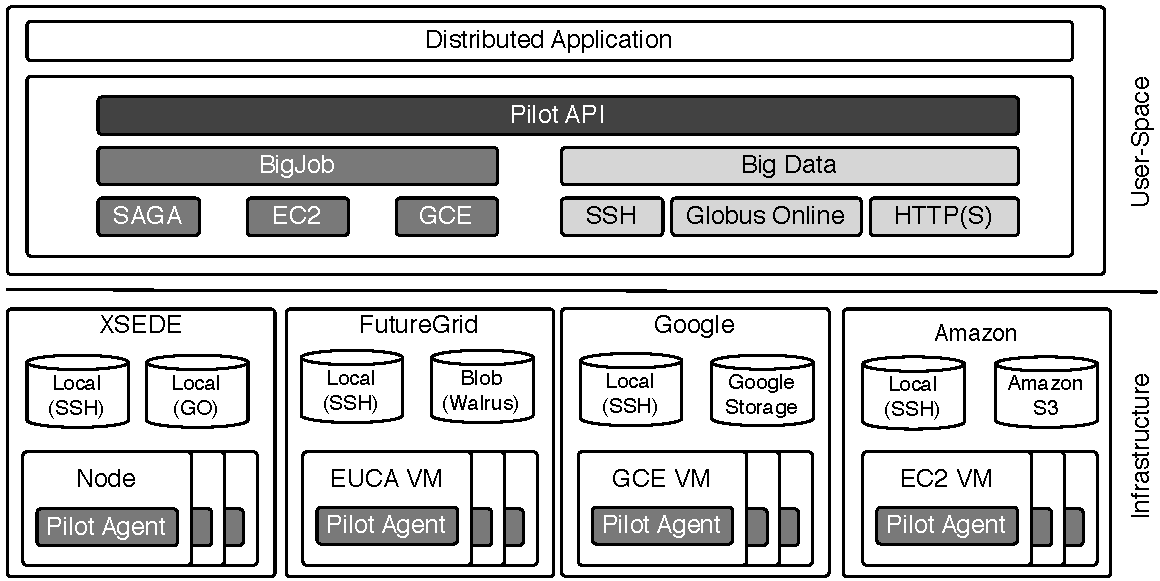
\includegraphics[width=0.7\textwidth]{figures/cloud_pilot_job.pdf}
                \caption{\textbf{BigJob Pilot Abstractions and
                    Supported Resource Types:} BigJob and BigData
                  provide a unified abstraction to compute and data
                  resources of both grid and cloud
                  environments. Resources are either accessed via
                  SAGA~\cite{ogf-gfd-90,saga-bliss-pd} or via a custom
                  adaptor.}
	\label{fig:figures_cloud_pilot_job}
\end{figure}


\begin{wrapfigure}{r}{0.4\textwidth}
	\upp\upp
	\centering
		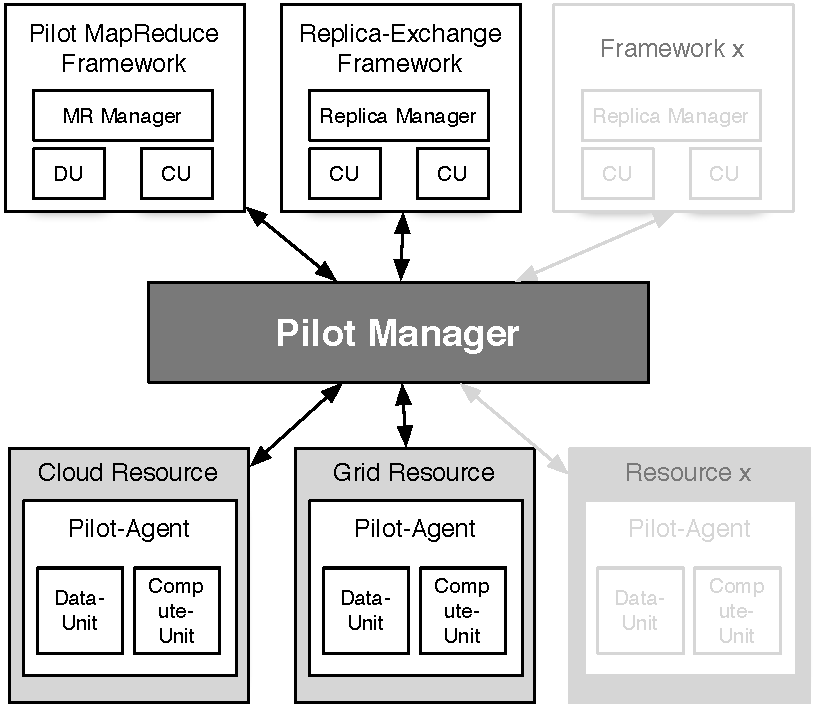
\includegraphics[width=0.4\textwidth]{figures/pilot-abstractions.pdf}
	\caption{\textbf{Pilot-Abstraction for Application-Level Resource 
	Management:}  \pilots are a well-proven abstraction for accessing 
	different types of storage and compute resources. Higher-Level framework, 
	such as Pilot-MapReduce or the Replica-Exchange~\cite{async_repex11} 
	can be built on these capabilities.}
	\label{fig:figures_pilot-abstractions}
\end{wrapfigure}

% The use of hybrid infrastructures presents a comprehensive approach to
% data-distribution to support large-scale data-analytics.


% \alnote{not sure what to do with that... It's not really different:
%   The specifics of matching \cus to clouds is distinct from the
%   matching \cus to grids.}\jhanote{previous comment put out of place?}


% \jhanote{Highlight
%   different scenarios in which grid-cloud interoperability would be
%   useful} \jhanote{By providing a uniform runtime environment, ie.
%   how do we handle grid-cloud affinity and thus reason about how to
%   move/distribute data... we attempt to provide a uniform distributed
%   cyberinfrastructure..} \jhanote{Need to go back and reference
%   introduction again, as well as the previous section on cloud data
%   infrastructure}

\subsection{Implementing the P* Model: BigJob and BigData}

The P* model~\cite{pstar12} is an attempt to provide the first minimal
but complete model for describing and analyzing \pilotjobs. We
particularly extended this model to \pilotdata (PD): PD provides
late-binding capabilities for data by separating the allocation of
physical storage and application-level \dataunits.  Similar to a
\pilotcompute, a \pilotdata provides the ability to create \pilots and
to insert respectively retrieve \dataunits. The
Pilot-API~\cite{pilot_api} provides an abstract interface to both
\pilotcompute and \pilotdata implementations that adhere to the P*
model.


% \alnote{Better P* introduction...}

\alnote{Bring CU, DU, VMs, pilot... How are VMs started through Pilot
  abstractions... - sequence chart?!}  


\alnote{Should we always refer to BigJob and BigData or just BigJob?}
\jhanote{not sure I understand.. stylistically or for consistency?
  I'd say completness and consistency: to be consistent:
  \pilot-Abstractions where general concept, \pilotjob, \pilotdata
  where concept and BigJob and BigData where specific}

Consistent with the P* model, BigJob
(BJ)~\cite{saga_bigjob_condor_cloud} and BigData
(BD)~\cite{Mantha:2012:PEF:2287016.2287020} provide a unified runtime
environment for \pilotcomputes and \pilotdata on heterogeneous
infrastructures (see Figure~\ref{fig:figures_cloud_pilot_job}). For
this purpose, BigJob provides a higher-level, unifying interface to
heterogeneous and/or distributed data and compute resources. The
framework is accessed via the \pilot-API~\cite{pilot_api}, which
provides two key abstractions: \pilotjob and \pilotdata. Applications
can specify their resource requirements using a \pilot
description. \pilots are started via the \pilotcomputeservice
respectively the \pilotdataservice.

\pilotjobs eliminate the need to interact with different kinds of compute 
resources, e.\,g.\ batch-style HPC/HTC resources as well as cloud resources, 
and provide a unified abstraction for allocating resources. Similarly, 
\pilotdata removing the need to interoperate with different data sources and 
stores, e.\,g.\ repositories, databases etc, by providing a virtualized data 
service layer, which can be used to allocated and access a heterogeneous set 
of data sources and stores.



Figure~\ref{fig:figures_bigjob-bigdata-architecture} shows the architecture of
BigJob/BigData. The \pilot-Manager is the central entity, which manages the
actual \pilots via the \pilot-Agent. Each agent is responsible for gathering
local information, for pulling \computeunits from the manager. The framework
relies on a central coordination service based on Redis~\cite{redis} for
communication between manager and agent.

\begin{wrapfigure}{r}{0.55\textwidth}
	\upp	\upp	\upp
	\centering
	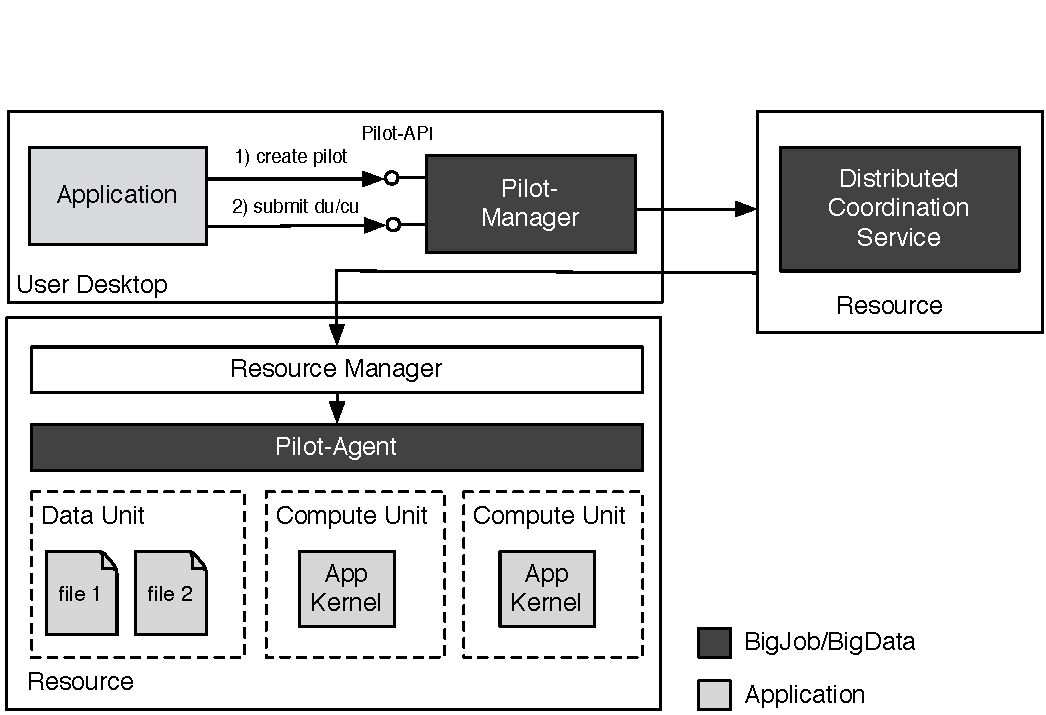
\includegraphics[width=0.55\textwidth]{figures/bigjob-bigdata-architecture.pdf}
	\caption{\textbf{BigJob and BigData Architecture:} The \pilot-Manager is 
	the central coordinator of the framework, which orchestrates a set of 
	\pilots. Each \pilot is represented by a decentral component referred to 
	as the \pilot-Agent, which manages the set of resources assigned to it. }
	\label{fig:figures_bigjob-bigdata-architecture}
\end{wrapfigure}

As shown in Figure~\ref{fig:figures_cloud_pilot_job} BigJob/BigData supports
various storage and compute resource types via a flexible plugin architecture.
For \pilotcomputes BJ supports various types of HPC/HTC resources via
SAGA/Bliss (e.\,g.\ Globus, Torque or Condor resources). Further, various
cloud plugins have been developed for supporting EC2-style backends as well as
Google Compute Engines. The plugin utilizes the native EC2 and GCE API for
launching the VM: for EC2 the Boto library~\cite{boto} and for GCE 
the Google Python API client~\cite{google-api-client} is used.
The EC2-API~\cite{amazonec2api} is the de facto standard for
managing VMs in clouds and can also be used for accessing different science
clouds, e.\,g.\ the Eucalyptus and OpenStack cloud of FutureGrid. Google
Compute Engine provides modern HTTP/REST/JSON and OAUTH for authentication.
Having started the VM, the \pilot-Agent is launched using SAGA and the SSH
adaptor of SAGA.

Similarly, a \pilotdata can be placed on different types of storage, e.\,g.\ a
local or remote filesystem or on object stores as often found in cloud
environments. Depending on the storage type different access respectively
transfer protocols are supported. For example, local/remote storage both on
grid and cloud resources can be managed via SSH. On production grid
infrastructures, such as XSEDE~\cite{xsede}, this kind of storage can also be
accessed via Globus Online~\cite{10.1109/MIC.2011.64}, which underneath relies
on GridFTP~\cite{ogf-gfd-20} for file movement etc. A particularity of cloud
environments are the described object stores. Object stores are typically
accessed via custom API typically based on HTTP/REST. For example, the Amazon
S3 API~\cite{amazons3api} is based on HTTP and XML and is also supported by
Eucalyptus Walrus and OpenStack Swift. Google Storage provides two APIs: an S3 
compatible and a JSON-based REST API. Again, Boto is used for S3-based storage 
resources and the Google Python API client for Google Storage. 

 
% \jhanote{unclear what HLA here implies} \jhanote{In general I think
%   this sub-section can be absorbed. We already have Section 3. Refer
%   to parts of it? Move some parts there?}


\subsection{Pilot-API: Managing Data and Compute Dependencies}

\pilot-Abstractions can marshal the difference between the different cloud
storage types and and provide a seamless, unifying environment to the
application simplify the usage of distributed infrastructures. Application can 
acquire resources in form of \pilots. A central \computedataservice is used to 
submit \computeunits (\cus) and \dataunits (\dus) to these \pilots. 
Application  can declaratively specify \cus and \dus and effectively manage 
the data flow between them. 


Figure~\ref{fig:figures_data-flow} shows the interactions and the data flow
between \computeunits and \dataunits. A \cu can have both input and output
dependencies to a set of \dus. BigJob and BigData will ensure that these
dependencies are met when the \cu is executed, i.\,e.\ either the \dus are
move to the \cu or the \cu is executed at (or close to) the location of the
\dus. The output files can be automatically transferred to a set of output
\dus. If a \cu declares a set of input dependency in the \texttt{input\_data},
the runtime system will then move the data to the working directory of the
\cu. Depending on the locality of the \du, this can be a local or remote
operation. BigJob/BigData uses an affinity-aware scheduler that ensures that
if possible ``affine'' \cus and \dus are co-located.

% Listing~\ref{lst:cu_du_dependencies} shows how these
% dependencies are specified on API-level.

\begin{wrapfigure}{r}{0.5\textwidth}
	\centering
		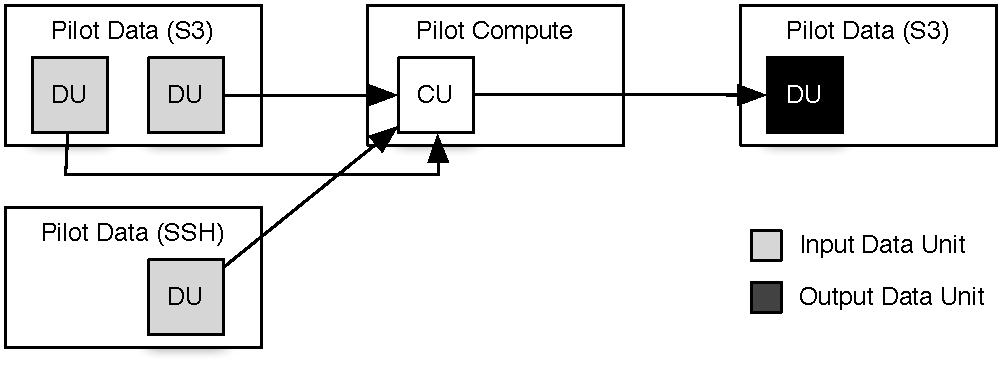
\includegraphics[width=0.5\textwidth]{figures/data-flow.pdf}
	\caption{\textbf{DU and CU Interactions and Data Flow:} Each \cu can specify a set of input \du (residing in potential different \pd). The framework will ensure that the \du is staged to the working directory of the \cu. Having terminated the job, the specified output is moved to the output \du.}
	\label{fig:figures_data-flow}
\end{wrapfigure}

% \begin{wrapfloat}{lstlisting}{r}{0.5\textwidth}
% \begin{lstlisting}[caption={{Managing \dataunit/\computeunit Dependencies}}, style=myPythonListing, label={lst:cu_du_dependencies} ]
% compute_unit_description = {
%          "executable": "/bin/cat",
%          "arguments": ["test.txt"],
%          "number_of_processes": 1,
%          "output": "stdout.txt",
%          "error": "stderr.txt",   
%          "input_data": [input_data_unit.get_url()],
%          # Put files stdout.txt and stderr.txt into output data unit
%          "output_data": [
%                          {
%                           output_data_unit.get_url(): 
%                           ["std*"]
%                          }
%                         ]    
% }
% \end{lstlisting}
% \end{wrapfloat}





\subsection{Affinities and Scheduling}
\alnote{
Distinguish data movement into cloud and intra cloud is important
No shared file system, but S3 as object store (cache)
}



\pilot-Abstraction provide the basis for application-level scheduling.
Applications can make placement decisions based on the \pilots it has
acquired. Additionally, applications can rely on an application-level
scheduling service as provided by BigJob and BigData. This service is exposed
via the \computedataservice interface and accepts both \cus and \dus. The
service decides how and when to place data and schedule its movement. 

\jhanote{first sentence is unclear, also maybe provide a brief
  definition of affinity first?} 

We use {\it affinities} to describe resource relationship between \cus, \dus,
and resources (i.\,e.\ \pilots). A simple model for describing such
relationships is used: data centers and machines are represented as a tree
(see Figure~\ref{fig:figures_affinities}). The further the distance between
two resources, the smaller the affinity. The framework relies on this affinity
description to efficiently manage the different kinds of storage as well as
distribution of data/compute across WAN.

% Each \pilot can specified the required affinity in it's description (see listing~\ref{lst:pilot_compute_affinity}).
% 
% \begin{code}[
% caption={Creation of a \textit{PilotCompute} on the specified  compute
% resource endpoint.},
% label={lst:pilot_compute_affinity}]
% pilot_compute_description = 
% {
%     "service_url":"s3://aws.amazon.com",
%     "number_of_processes": 1,                             
%     "working_directory": "/tmp/pilot-compute/",
%     "affinity_datacenter_label": "us-east-1a"              
% }
% \end{code}


\begin{wrapfigure}{r}{0.5\textwidth}
	\centering
		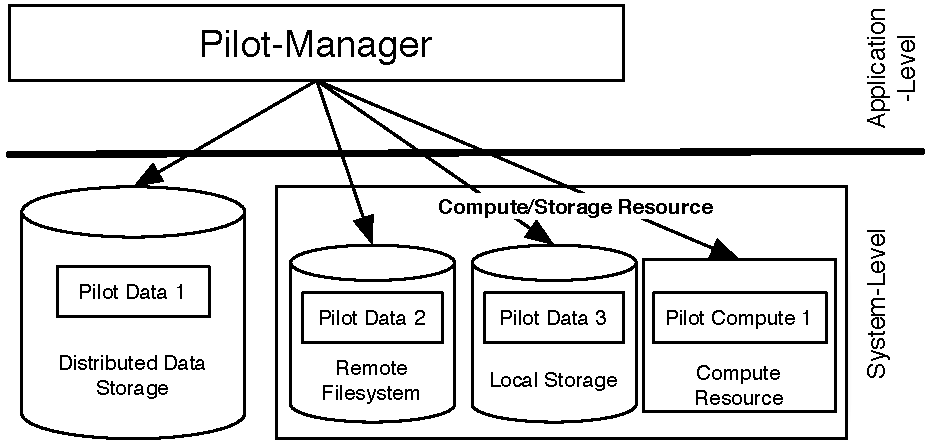
\includegraphics[width=0.48\textwidth]{figures/storage-types.pdf}
                \caption{\textbf{Pilot-Compute and Pilot-Data on Different
                                Types of Storage Resources:} BigJob/BigData 
				supports various types of resources. Affinities allow the user 
				to describe the 
				relationship between different types of resources enabling the 
				scheduler to efficiently make placement decisions. }
	\label{fig:figures_storage-types}
\end{wrapfigure}

As explained before, even within a single cloud, managing data locality is a
great challenge due the various storage options.
Figure~\ref{fig:figures_storage-types} summarized the different kinds of
storage options an application has to manage. \pilot-Abstractions not only
provide a uniform interface to these different kinds of storage, the also
support application-level scheduling. The core of the \pilot-Manager is an
affinity-aware scheduler. BigJob and BigData support different forms of
data/compute affinities via the \computedataservice. The internal scheduler of
the \computedataservice relies on affinity as first entity to describe
relationships between \dus, \cus and resources. Affinities are an essential
tool for modeling the different storage characteristics and to allow an
effective reasoning about different storage topologies and data/compute
placements. BJ relies on affinity label for describing resource topology.


Every \pilot is assigned an affinity label in the resource description.
Affinities are organized in an hierarchical way.
Figure~\ref{fig:figures_affinities} shows e.\,g.\ how a distributed system
consisting of different types of cloud and grid resources can be modeled. The
shorter the distance between two nodes, the higher the affinity. Commercial
clouds, such as Amazon and Google, are typically organized into geographic
regions. Within each region multiple availability zones exist. Commonly, data
movements between the lower-level availability zones are cheap and fast, while
movements between regions costs some significant amount on money and time.
Even worse are movements between infrastructure, e.\,g.\ between Amazon,
Google and FutureGrid. Both \cus and \dus can request a certain affinity. The 
runtime system then ensures that the data and compute affinity requirements of 
the \cu/\du are met.


\begin{figure}[t]
	\centering
		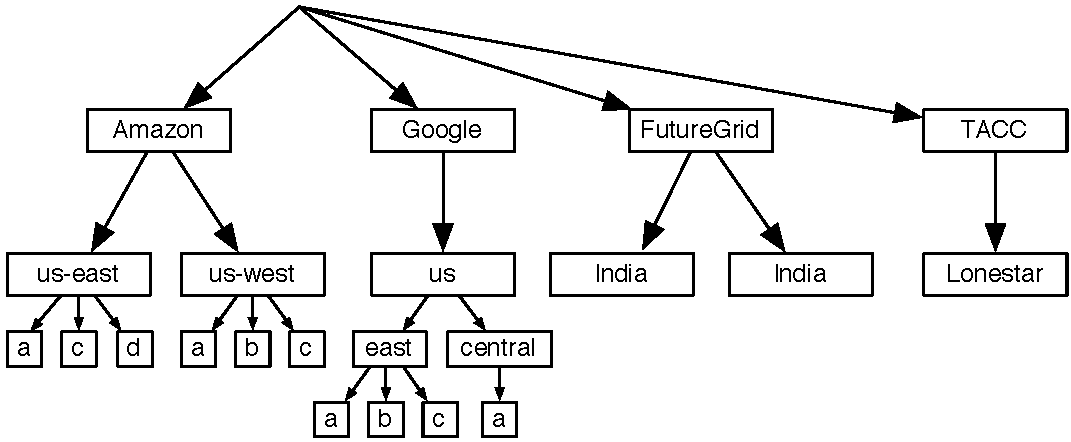
\includegraphics[width=0.6\textwidth]{figures/affinities.pdf}
	\caption{\textbf{Managing Affinities between Cloud and Grid Resources:} 
	\pilotdata assigns each resource an affinity based on a simple 
	hierarchical model. The smaller the distance between two resources, the 
	larger the affinity.}
	\label{fig:figures_affinities}
\end{figure}

Each of the storage types in Figure~\ref{fig:figures_storage-types} can be 
assigned an affinity. The model is able to deal with subtle differences 
between clouds and grids/clouds. For example, at Amazon S3 is service that is 
confined by a single region, while Google Storage spawns multiple regions.

The \computedataservice scheduler matches the affinity requirements of
a \cu/\du with the available set of resources before assigning it to a
\pilot.  \cus are placed closed to a \du. Before a \cu is actually
run, the \du is exported to the working directory of the \cu. In the
cloud cases e.\,g.\ this means that the data is copied from an object
store to the local filesystem where the \cu runs.

Having discussed how \pilots are a good abstraction for resource
effective application-level resource management. Using this high-level
abstraction to computing and storage resources, higher-level
frameworks can as depicted in
Figure~\ref{fig:figures_pilot-abstractions} request resources
(\pilots), on which they then can run tasks (\computeunits). Thus,
\pilots can be used as basis for building capabilities on
grids/clouds; Pilot-MapReduce is a good example for this (see
section~\ref{sec:pmr}).

\section{Pilot-MapReduce for Clouds}
\label{sec:pmr}

Pilot-MapReduce (PMR)~\cite{Mantha:2012:PEF:2287016.2287020} is a \pilot-based
implementation of the MapReduce programming model, which decouples the
logic/pattern of MapReduce from the actual management of the compute, data and
network resources. For this purpose, PMR efficiently reuses the resource
management and late-binding capabilities of BigJob and BigData via the 
\pilot-API interface. Another key feature of the \pilot-API is the ability to 
declaratively define the data flow between the \dataunits and \computeunits. 
Based on the defined affinities, the scheduler will then attempt to place data 
and compute as close as possible. If necessary, data will be moved. 

Using the \pilot-Abstractions, applications such as PMR can transparently use
different kinds of grid and cloud resources, e.\,g.\ Amazon EC2/S3, Google
Compute Engine/Storage and Eucalyptus-based science clouds. Details specific
to the respective resource type are hidden behind the \pilot interface
enabling the application to focus on the definition and management of the
workload in form of \cus and \dus.

PMR exposes an easy-to-use interface, which provides the complete
functionality needed by any MapReduce-based application, while hiding the more
complex functionality, such as chunking of the input, sorting the intermediate
results, managing and coordinating the map and reduce tasks, etc. The user
solely has to provide an implementation of the chunk, map and reduce function
in form of a executable script.

\subsubsection*{Architecture and Interactions:}

\begin{figure}[t]
	\centering
    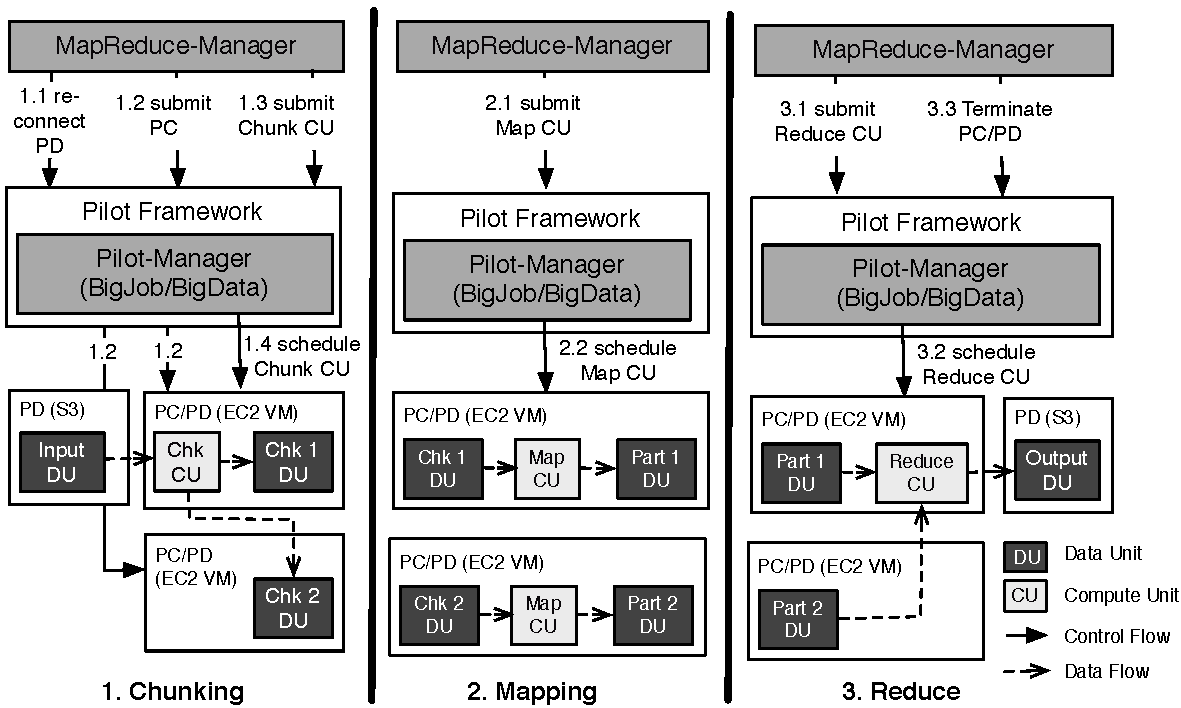
\includegraphics[width=0.95\textwidth]{figures/pmr_clouds_flow.pdf}
    \caption{\textbf{Pilot-MapReduce Control and Data Flow:} PMR allocates 
     both storage and compute resources via the \pilot-API. The three stage 
    MapReduce run is then managed by submitting \dataunits and \computeunit to 
    the \pilot-Manager. The \pilot-framework takes care of moving the data in 
    and out the different stages.}
	\label{fig:figures_pmr_clouds}
\end{figure}

Figure~\ref{fig:figures_pmr_clouds} shows the architecture of the
\pilotmapreduce framework. The flow of a MapReduce run involves the (i) the 
chunking of the data, (ii) the execution of the map compute tasks, and (iii) 
the execution of the reduce task. Between the stages data must be moved. 
Between stage (ii) and (iii) the data is sorted and moved; this stage is also 
referred to as shuffling.

PMR allocates both storage and compute resources
using BigJob/BigData. This enables PMR to support a heterogeneous set of
cloud/grid resources (cmp. Figure~\ref{fig:figures_cloud_pilot_job}). Having
spawned a set of\pilots, PMR can flexibly utilize them for executing chunking,
mapping and reduce tasks as well as for managing the data flow between the
phases. For this purpose, the framework solely needs to declare the input and
output data dependencies for a \computeunit. BigJob/BigData will then attempt
to place the \computeunit close to the input data. This practice is applied to
the input as well as the intermediate data of the different stages.


The scenario depicted in Figure~\ref{fig:figures_pmr_clouds} shows a MapReduce
flow on Amazon's cloud infrastructure. Typically, in cloud environments, the
data is initially stored in a low-cost object storage, such as S3. In step 1.1
the framework re-connects to the S3-based \pilotdata. Then, the \mrmg spawns a
set of \pilots for executing the computational tasks. Each \pilot is
represented by a VM. In stage 1, the initial data is downloaded to the VM and
then chunked into multiple \dus. For this purpose, a chunk \du is executed on
a \pilot. The chunk \du downloads the declared input data from the S3
\pilotdata and splits it into a set of output \dus (which are in this scenario
directly located on the VM). Then a map \cu is executed on each of the \dus.
Each \cu creates an output \du containing the result of the map phase, i.\,e.\
the partitioning files. Finally, the reduce \cu is executed and the output is
written back to a defined S3-based \pilotdata.


% difference to grids
On grids, the \mrmg allocates a set of compute and data resources by starting
one (or most often a set of) \pilotdata and \pilotcompute on different
resources mainly using SAGA/Bliss~\cite{saga-bliss-pd} as abstraction to the
local queuing system. In general, on each resource one \pilotcompute and one
\pilotdata are co-located. In contrasts to clouds, most grid resources have a
shared file systems that simplifies in particular the management of the input
data.


% The
% data pilot is either created with reference to local input data or the input
% data is moved to the data pilot after its creation.
% On clouds, the \mrmg allocates compute pilot for each virtual image instance
% and a single data pilot for the entire cloud storage. This cloud storage acts
% as a central storage of entire input, temporary and intermediate data which is
% accessed by the compute units launched by compute pilots in map and reduce
% phase. The data generated by compute units in chunk, map and reduce phases is
% directly written to cloud storage via Pilot-Data from the VM. The performance
% of PMR on clouds depends on the bandwidth and data transfer rate between the
% cloud storage and the VM, and hence depends on the locality of cloud storage
% and the VM.


\subsubsection*{Distributed MapReduce:}

Often, there are MR-based applications that to operate on distributed
data, including but not limited to distributed scenarios as
represented by different clouds or regions within a single cloud,
clusters connected over WAN, or production distributed
cyberinfrastructure such as XSEDE. Data distribution can be difficult
to manage for performance, as latencies and bandwidths may vary
unpredictably.

\pilotmapreduce provides a flexible, extensible implementation of MR:
\pilotdata can be spawned to various (possibly distributed)
resources. The affinity-aware scheduler attempts to co-locate
compute/data using the minimal amounts of data movements necessary. We
previously showed ~\cite{Mantha:2012:PEF:2287016.2287020} how these
capabilities can be used to support different distributed MapReduce
topologies, e.\,g.\ distributed and hierarchical MapReduce
configurations. A distributed PMR utilizes multiple resources often to
run map tasks close to the data to avoid costly data transfers; the
intermediate data is then moved to another resource for running the
reduce tasks. In a hierarchical PMR the outputs of the first complete
MapReduce run are moved to a central aggregation resource. A complete
MapReduce run is then executed on this resource to combine the
results.
 






\alnote{Add layered diagram (incl. PMR) of software stack for different 
infrastructures}

\alnote{TODO: Can we add a paragraph on distributed MapReduce. Maybe extending 
figure 6 to a more distributed or heterogeneous scenario}


\section{Experiments}

The aim of this section is to demonstrate how BigJob/BigData can be used to
interoperable access different types of compute and storage resources. We show
how BigJob/BigData can support interoperability in a highly fragmented cloud
environment consisting of various commercial and science cloud infrastructures
with different interfaces and characteristics. In particular, we focus on
aspect related to infrastructure for data-intensive applications and novel
services such as object stores (that are commonly not available in traditional
grid resp. HPC environments). Further, we illustrate representative usage
modes of \pilot-Abstractions and show how they can support
frameworks such as Pilot-MapReduce. For this purpose, we run several
experiments on FutureGrid (FG) and various cloud infrastructures, including
the Eucalyptus cloud on India/FutureGrid, Amazon EC2 and Google Compute
Engine. Each experiment is repeated at least five times.

\alnote{Further possible goals: show elasticity, dynamic resource usage}

\jhanote{We need a few sentences that states why we chose the
  experiments that we did, why they in an abstract sense validate our
  claims of pilot-abstractions for clouds and bigdata.  And last but
  not least why the set of experiment is necessary and sufficient to
  make the claim..  ie. we need a few sentences explaining the design
  and rationale of experiments.}
	
\subsection{Objective 1: Interoperability}
\label{sec:perf_interop}
\note{Objectives: basic interoperable; determine basic characteristics of 
different infrastructures}

To validate the effectiveness and usability of the Pilot-API/BigJob/BigData,
we conducted a series of experiments on various cloud infrastructures. In 
particular, we focus on evaluating the interoperability of the different 
storage and compute services offered by the different infrastructures.
We show how the \pilot-API allows the effective management of data and data 
transfers. Further, it provides application a powerful tool to trade-off 
different infrastructure characteristics. 

In the following, we focus on the most common usage modes of clouds: 
Initially, files are moved to a cloud-based storage services. From there the 
data is made available to the VMs for running computations. Commonly, files 
are moved only once to the cloud. As part of this evaluation, we investigate 
both the transfer both to and within the cloud infrastructure. We use the 
FutureGrid machines Hotel and India as submission machine, i.\,e.\ the machine 
where the initial data resides and the \pilots are submitted from. We 
investigate different scenarios: In scenario (a) we investigate the influence
of the input data size on the overall runtime; in scenario (b) we analyze
different infrastructures configurations.

\begin{figure}[t]
    % \begin{subfigure}[b]{0.5\textwidth}
	\centering
		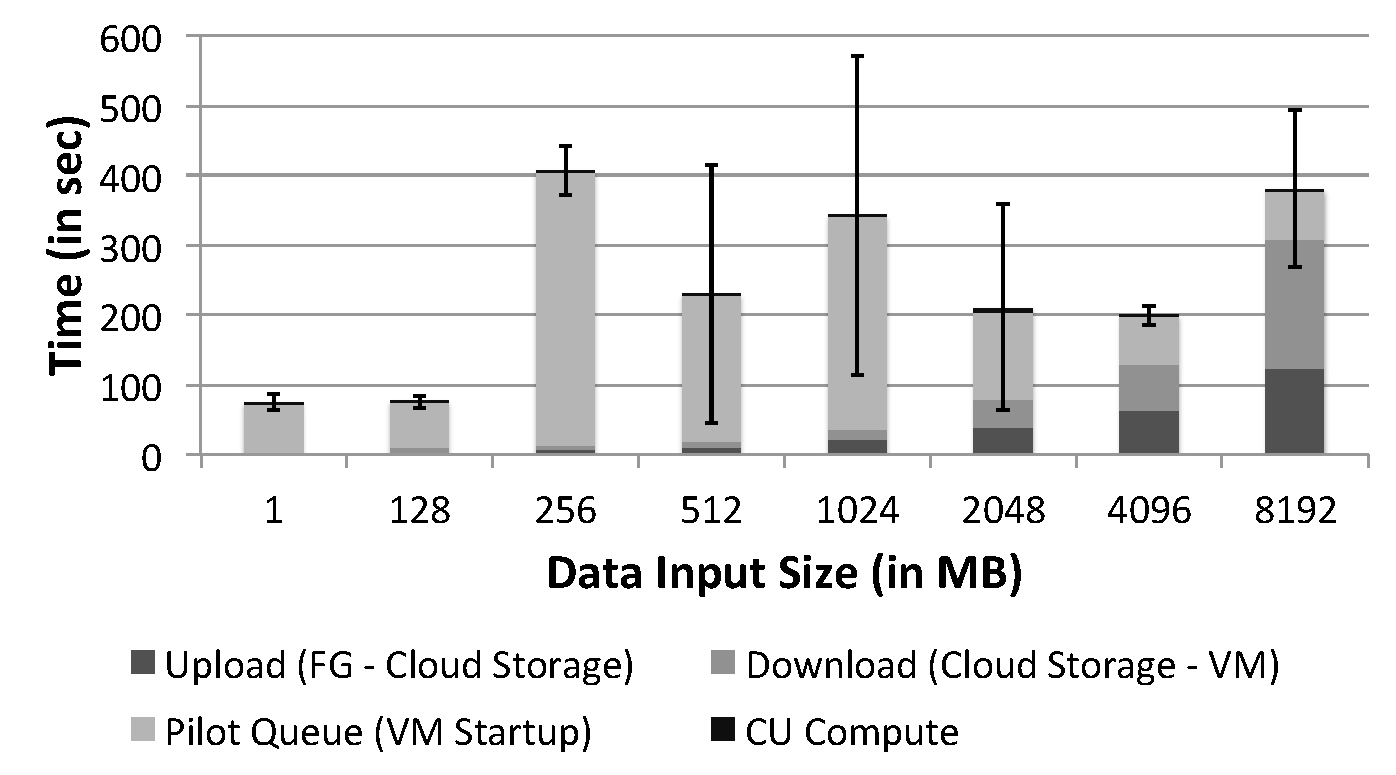
\includegraphics[width=0.9\textwidth]{performance/pd_fg_input_size.pdf}
	\caption{\textbf{Dependence on Input Data Size 
	(FutureGrid/Eucalyptus/Walrus on India):} With the increasing amount of 
	data both the time to upload the files to the cloud and the the time to 
	download to the VM increases. Note that the VM startup time (observable in 
	the \pilot queue time) depends on external factors, in this case the 
	current utilization of the Eucalyptus cluster.}
	\label{fig:performance_size}
   % \end{subfigure}
   %    \begin{subfigure}[b]{0.5\textwidth}
   	% \end{subfigure}
\end{figure}

\alnote{make sure b1 is reflected in a. many variables (not all of them are 
controlled, different variation of how infrastructure manage data); make 9b as 
log}

Figure~\ref{fig:performance_size} shows the results on scenario (a). For this
scenario, we utilize the Eucalyptus VM and Walrus service on India. The 
initial dataset resides on India. As expected, the runtime increases with the 
increasing amount of data. Both the data upload time to cloud and download 
time within the Eucalyptus cloud increase linearly. As all transfers are done 
in a local network this is an expected result. Also, we observed a high 
fluctuations in the VM startup times, which can be observed in the \pilot 
queue times. This is caused by externally controlled factors, most likely
the current utilizations of the Eucalyptus cluster (the data was 
collected over a period of week). In general, the \pilot queue time varies on 
India between 1 and 10\,min.

\begin{figure}[ht]
    % \begin{subfigure}[b]{0.5\textwidth}
	\centering
\centering
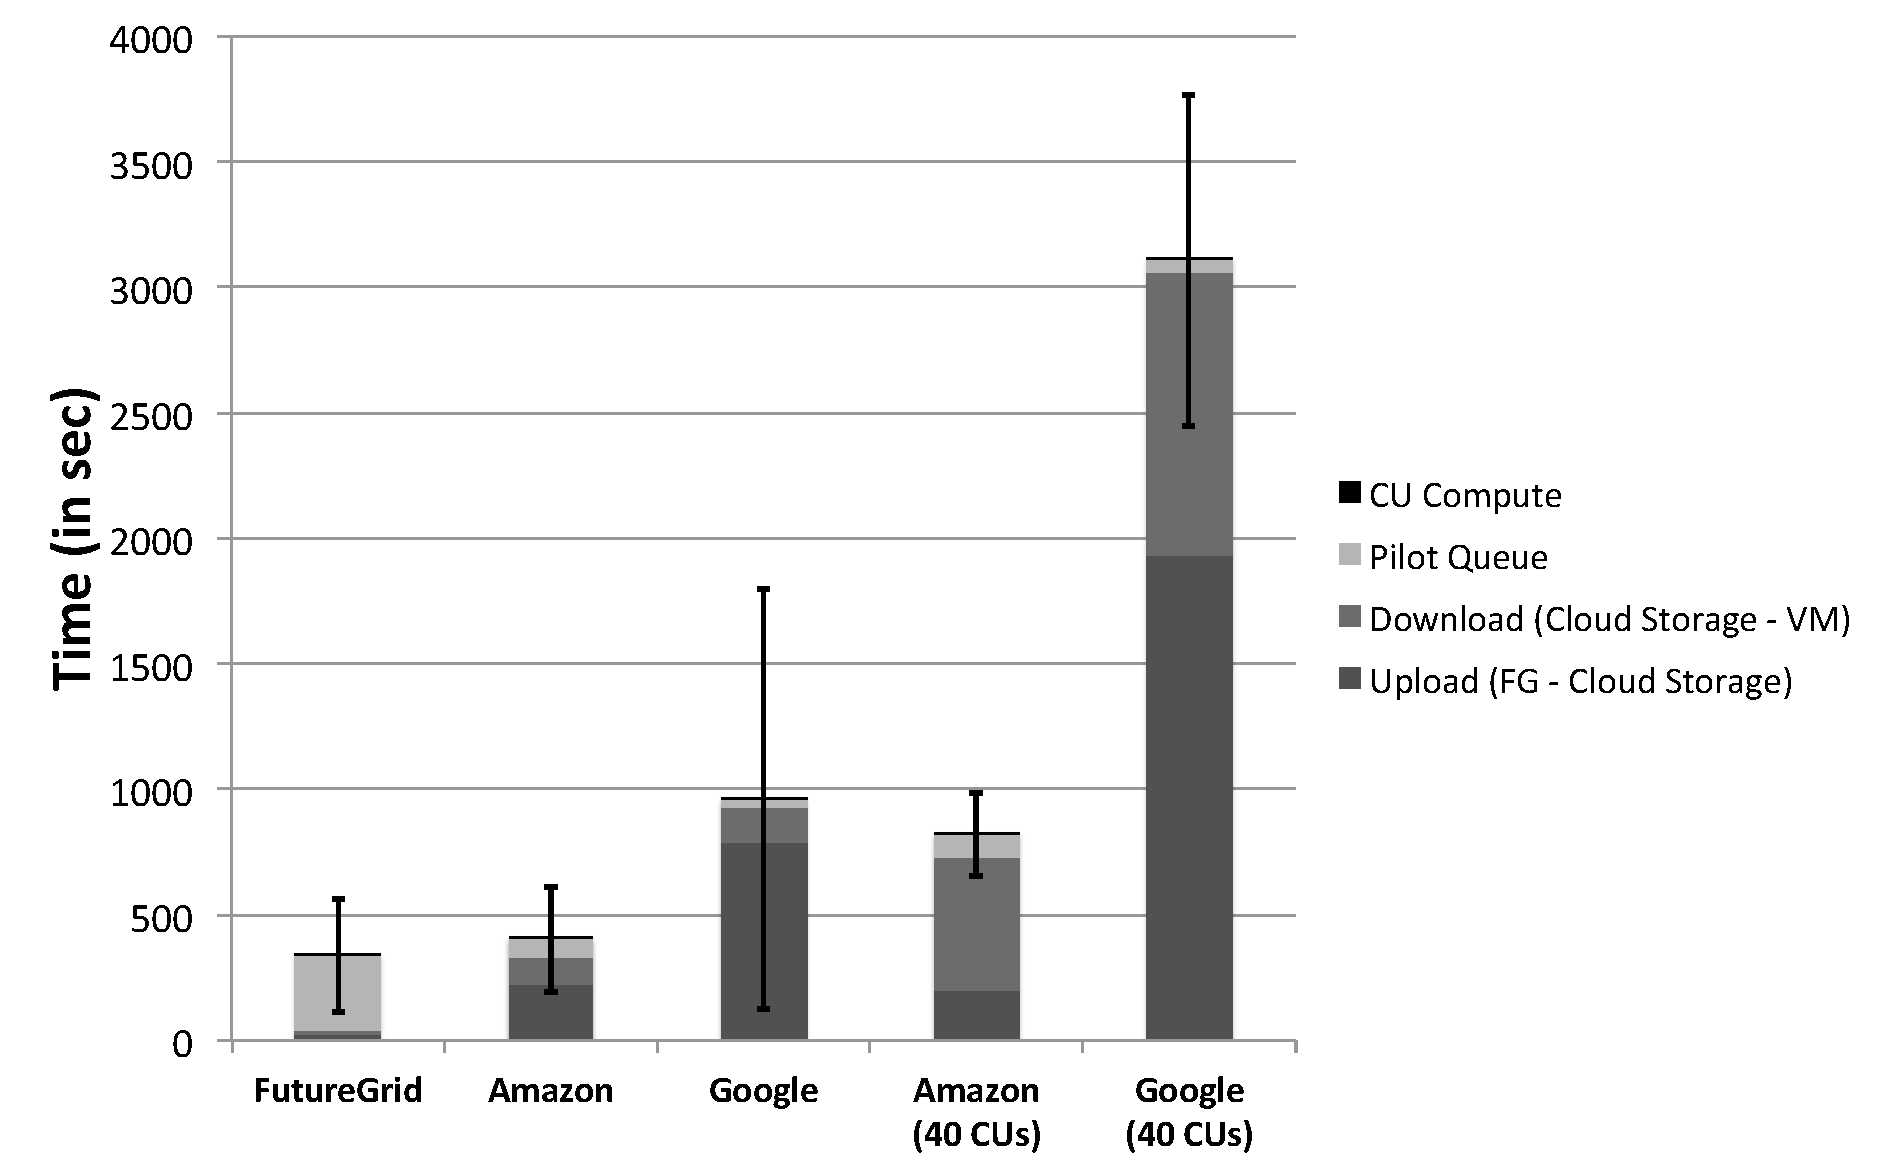
\includegraphics[width=0.9\textwidth]{performance/pd_google_aws.pdf}
\caption{\textbf{BigJob/BigData on Different Infrastructures:} BigJob/BigData
supports different commercial and science cloud infrastructures each with its
own types of storage and compute services. In scenario (b1), (b2), (b4), (b6)
we execute 1\,\cu; in scenario (b3), (b5) and (b7) we run 5\,\cus per VM core
to test the available connectivity between VM and cloud storage. A
critical factor in particular for the commercial clouds of Amazon and Google
is the available bandwidth for the data ingest. }
\label{fig:performance_pd_google_aws}
\end{figure}


In scenario (b) we investigate the execution of different
workload/infrastructure configurations with a constant input \du of size
1\,GB. Figure~\ref{fig:performance_pd_google_aws} shows the results. Scenario
(b1) - (b3) show different configurations on FG/India: in (b1) and (b2) we
compare different \pilotdata backends (Eucalyptus Walrus and SSH) on the same
resources. In both cases we upload the 1\,GB input file to the Walrus resp.
SSH-based storage. We then execute 1\,\cu that downloads the data prior its
execution. While the initial upload to the Walrus respectively SSH \pilotdata
is comparable, the download to the VM time with SSH is considerable slower
than for Walrus. In general SSH is associated with additional overheads caused
e.\,g.\ by the encryption, in particular when compared to the HTTP-based
Walrus protocol. Again, the \pilot queue was highly unpredictable and dominate
the overall runtime in these scenarios. In (b3) we execute in total execute 
20\,\cus (up to 4 concurrently) each of them downloads the input data from the 
Walrus \pd. While the initial data is only uploaded once, it obviously leads 
to a significant increase in the download time indicating that the available bandwidths to the cloud storage might have been saturated.

The cloud scenarios (b4) - (b7) are dominated by the data ingest phase
(i.\,e.\ the upload time). Typically, data movement into the cloud are slower
and more expensive than intra-cloud data movements. In this particular
scenario the data ingest time for clouds varies between $\sim$4\,minutes for
Amazon and $\sim$18\,minutes for Google. The primary determinant of this time
is the available Internet bandwidth. While the upload performance is
determined by external factors (currently utilization of the Internet
connection), in the investigated scenario the data transfer time is
consistently higher for Google Compute Engine than for Amazon. The external
dependency on Internet bandwidth is the high standard deviation (that is
mainly caused by the data ingest phase). Also, it must be noted that Amazon
gives you more option to select a location for your data -- in this scenario
the region us-east, which is close to the hotel resource, was used. For Google
Storage it is only possible to select between the US and Europe. Once the data
is uploaded to the cloud, it can be re-used multiple times. Usually, the cloud 
providers ensure that a suitable link between VM and cloud storage exists.

The \pilot queue time (which includes the VM startup time), GCE is faster than
Amazon EC2. Also, the available intra-cloud bandwidths are better for GCE: The
data download time for GS/GCE is about 40\,\% faster than for S3/EC2 in the
single \cu case. However, the bandwidth available at GCE saturates fast with
8\,\cus concurrently downloading the input data: the download time in the
multi \cu scenario is 12 times slower on GCE compared to a slowdown of only 5
times on Amazon. Also, the \cu execution time are significantly lower on GCE.
In both cases the smallest possible VM was used; however, it must be noted
that Amazon's t1.micro instance type doesn't provide any guaranteed CPU time.
Also the memory is with 613\,MB considerable smaller than for Google's
smallest VM n1-standard-1, which has 3.75\,GB memory.




\subsection{Objective 2: Support of Higher-Level Frameworks}

In this section, we show how higher-level frameworks -- in this case
Pilot-MapReduce -- can benefit from the usage of \pilot-Abstractions. For this
purpose, we utilize the Amazon EC2/S3 services for running a genome sequencing 
MapReduce application with PMR (GS/PMR). 

\begin{figure}[ht]
\centering
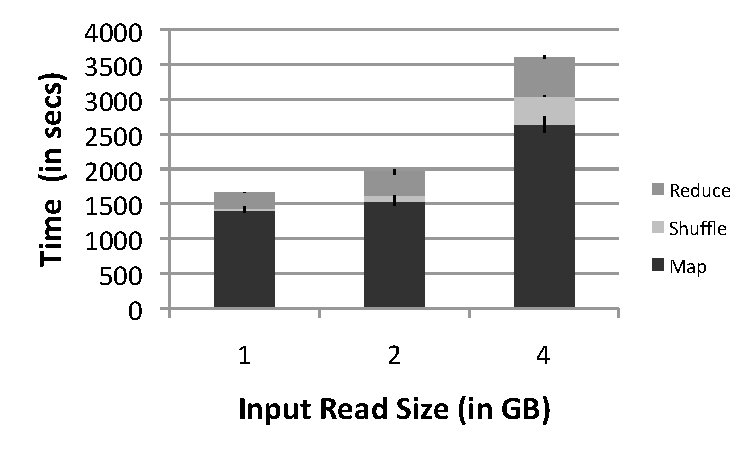
\includegraphics[width=0.7\textwidth]{performance/pmr_cloud.pdf}
\caption{\textbf{PMR on Clouds:} The figures show the results of different PMR 
runs on EC2. The input data has been initially moved to S3. As expected, the 
runtime increases with the input size, which is consistent with earlier 
results~\cite{Mantha:2012:PEF:2287016.2287020}. The observed fluctuations are generally very low (compared to the overall runtime).
}
\label{fig:performance_pmr_aws}
\end{figure}


The GS/PMR is a Pilot-MapReduce based Seqal
~\cite{Li:2010:FAL:1741823.1741825, Mantha:2012:PEF:2287016.2287020}
application. It performs an important part of the sequencing
workflow. The application implements the read alignment in the mapping
phase using BWA aligner~\cite{Li:2010:FAL:1741823.1741825} and
duplicate read removal in reduce phase using Picard’s rmdup
~\cite{picard}. The GS/PMR reducer removes duplicate reads based on
the key fields-chromosome, position and strand of the mapper output.

For experiments demonstrating the utilization of \pilot-Abstractions for
\pilotmapreduce, we utilize a large Amazon VM (type: m2.4xlarge) as well as
different sets (1\,GB, 2\,GB, 4\,GB) of input data, which has been initially
transferred to Amazon S3. PMR also uses a S3-\pd to store in the necessary 
chunk, reducer and mapper scripts. The application re-connect at the beginning 
to this data using the \pd URL. Consistent we earlier experiments, the upload 
to the S3 \pd requires between $\sim$2.5\,minutes for the 1 GB and $\sim$10\,minutes for the 4\,GB scenario. 

We run a total of 8 MapReduce workers and utilized a chunk size of
475740 short reads. Results are plotted in Fig.~\ref{fig:performance_pmr_aws}. 
The experiment is repeated three times, with experiment-to-experiment
fluctuations in time relatively small (compared to actual values). The time 
for launching the \pilot, which includes the VM startup time, is about 
$\sim$3\,minutes. Consistent with Ref.~\cite{Mantha:2012:PEF:2287016.2287020}, 
the reduce phase increases essentially linearly with input data size. The 
intermediate data that needs to be moved to the reduce task is about 1.8 as 
large as the input data.

% \begin{itemize}
% 	\item grid only
% 	\item cloud only
% 	\item grid / cloud concurrently
% 	\item  Different amounts of intermediate data: 1GB, 10GB, 100GB, 1000 GB	
% \end{itemize}

\section{Conclusion and Future Work}

\pilot-Abstractions enable the efficient interoperable usage of
different kinds of resources. We show how a large set of heterogeneous
set of both commercial and scientific cloud resources can be accessed
via the \pilotcompute and \pilotdata Abstraction. Further, we
established affinities as a powerful abstraction for describing
relationships between compute, data and resources. We showed that
affinities can be used to model distributed resource topologies
consisting of heterogeneous cloud resources.  \pilot-Abstractions
provide the basis for implementing higher-level, distributed
frameworks, which can support different programming, e.\,g.\ PMR
provides a \pilot-based implementation of the MapReduce programming
model.

This paper contributes to the practice and experience of distributed
systems for data-intensive computing by validating and extending the
\pilot-Abstraction --- a highly successful, but arguably under
utilized runtime environment in distributed computing, to cloud
infrastructures. We believe there remain a plethora of important
research questions that we do not touch upon here, but for which we
believe that \pilot-Abstractions will provide a useful vehicle to
research.

\alnote{Extend to other data-intensive abstractions: all-pairs, stream
  processing;OCCI; dynamic execution}

\section*{Acknowledgements}
\footnotesize{This work is funded by NSF CHE-1125332 (Cyber-enabled
  Discovery and Innovation), HPCOPS NSF-OCI 0710874 award, NSF-ExTENCI
  (OCI-1007115).  Important funding for SAGA has been provided by the
  UK EPSRC grant number GR/D0766171/1 (via OMII-UK) and the Cybertools
  project (PI Jha) NSF/LEQSF (2007-10)-CyberRII-01, NSF EPSCoR
  Cooperative Agreement No. EPS-1003897 with additional support from
  the Louisiana Board of Regents.  SJ acknowledges the e-Science
  Institute, Edinburgh for supporting the research
  theme. ``Distributed Programming Abstractions'' \& 3DPAS. 
  This work has also been made possible
  thanks to computer resources provided by TeraGrid TRAC award
  TG-MCB090174 (Jha). This document was developed with support from
  the US NSF under Grant No. 0910812 to Indiana University for
  ``FutureGrid: An Experimental, High-Performance Grid Test-bed''. We
  thank FutureGrid support, in particular Fugang Wang for exceptional
  support. Last but not least, we thank our fellow Radicalistas for
  their support and input.}

\bibliographystyle{wileyj}
\bibliography{literatur,local,saga-related,saga}

\end{document}
